\documentclass[a4paper, 12pt]{scrreprt}

\pagenumbering{roman}
\setcounter{secnumdepth}{3}
\setcounter{tocdepth}{2} 

\usepackage[german]{babel}
\usepackage[utf8]{inputenc}
\usepackage[T1]{fontenc}
%\usepackage{fancyhdr}
\usepackage{geometry}
\usepackage{lmodern}
\usepackage{verbatim}
\usepackage{graphicx}
\usepackage[hyphens]{url}
\usepackage[pdfborder={0 0 0}]{hyperref}
\usepackage{listings}
\renewcommand\_{\textunderscore\allowbreak}
\usepackage{float}

\usepackage{caption}

\usepackage{amsmath}
\usepackage{blindtext}


\usepackage{fancybox}
\usepackage{makeidx}% \makeindex
\usepackage{lastpage}
\usepackage{natbib}

%\linespread{1.5}
%\geometry{footskip=40pt}
\setcounter{page}{2}
\linespread{1.25}


\begin{document}

\begin{titlepage}
%\includegraphics[scale=0.3]{Z1.png} \hfill
%\includegraphics[scale=0.1]{2.png}\\[1.8cm]
    \begin{center}
    \LARGE \textbf{VirtualDesktop} \\
    \vspace{2.5cm}
    \large\textbf{Projekt}\\
    \vspace{2.5cm}
    \normalsize
    Hochschule RheinMain Wiesbaden \\
    \vspace{2cm}
    \large \textbf{Fortgeschrittene Themengebiete der Informatik\\ Cloud Computing\\}
    \vspace{1cm}
    \normalsize
    Abgabedatum: 30. Januar 2019\\
    \vspace{2.7cm}
    \end{center}
 \normalsize{
    \begin{tabular}{ll}
    	Gruppe: & \\
    	Robin Bergfeld & \\
    	Abiram Pakeerathan & \\
    	Simon Rininsland & \\[0.5cm]
    	Dozent: &\\
        Prof. Dr. Philipp Schaible & \\
    \end{tabular}
    }
\end{titlepage}



\clearpage
\tableofcontents
\clearpage

\pagenumbering{arabic}

%zitieren:
% \cite{Joa10:1}

\chapter{Einführung}
%Mit was, wer wo...
Im Rahmen des Moduls Cloud Computing an der Hochschule Rhein Main im Wintersemester 2018 / 2019 bei Prof. Dr. Schaible eine Web-Anwendung unter Verwendung von Amazon Web-Services (AWS) entwickelt worden. Zunächst wird in diesem Kapitel die Idee vorgestellt, anschließend wird die Architektur und die Umsetzung thematisiert.

\section{Projektanforderungen}
%- Welche Anforderungen vom Modul\\
%- Fokus des Projekts
Es ist eine Web-Anwendung unter Verwendung von Amazon Web-Services (AWS) zu
entwickeln, die mindestens folgende Funktionalitäten beinhalten soll.
\begin{enumerate}
\item Eine statische Web-Seite als Startpunkt der Anwendung.
\item Ausgelagerte REST APIs für dynamisches Verhalten der Anwendung.
\item Benutzerverwaltung mit expliziten Authentifizierungs- und Autorisierungsverwaltung.
\item Die Daten der Anwendung sollen in einer Datenbank verwaltet werden. Die SQL und NoSQL Datenbanken sollen dabei passend eingesetzt werden.
\item Die Anwendung soll mit heterogenen Daten umgehen können. Zusätzlich zu den
organisatorischen Daten (Nutzerverwaltung, Anwendungslogik, etc.) müssen
Multimedia-Daten (Bilder, Audio, Video) integriert werden. Es muss dabei möglich
sein, die Multimedia-Daten entweder herunterzuladen oder zu streamen.
\item Die Anwendung muss horizontal skalierbar sein. (Begründung!)
\end{enumerate}
Zusätzlich haben wir eigene Projektanforderungen hinzugefügt:
%todo vieleicht auch, dass es unsere Entwickler aufgaben sind. Umschreiben wieso, der Zweck wer, mehr soll
\begin{enumerate}
\item Auslegung auf spätere Socketnutzung.
\item Der Code liegt in einen öffentlichen Repo.
\item Der Stack ist von jedem Deploybar. Keine statischen Variablen. Der Stack soll mit einen Befehl aufgebaut werden.
\item Trennung von Model, View und Controller. 
\item Die NodeJS Funktionen sollen möglichst parallel laufen, um wartende Funktionen zu vermeiden.
\item Die EC2 Instanz speichert keine Dateien, sondern \dq schleust\dq\ sie nur durch.
\end{enumerate}

\section{VirtualDesktop}
%- Was mit Bildern (kurz, vielleicht nur ein Bild)\\
%- Funktionen erläutern (MultiWindow, Benutzerverwaltung inkl Rechteverwaltung, Stream, Up-Download, Show)\\
%- Ziel des Produkts (müssen sich mit Anforderungen des Moduls decken)\\

Die Web-Anwendung \textit{VirtualDesktop} soll registrierten Benutzern virtuelle Desktops zur Verfügung stellen, die auf jedem Gerät aufrufbar sind und mit anderen Benutzern geteilt werden können. Die erstellten Desktops sollen zur Multimediaablage genutzt werden. Der Up- und Download ist mit beliebigen Dateitypen möglich. Zusätzlich können Bilder angezeigt sowie Audio- und Video-Daten gestreamt werden.\\[0.25cm]
Alle Benutzer müssen sich anmelden um die Anwendung nutzen zu können. Ein Benutzer kann mehrere Desktops anlegen und diese verwalten. Das Anlegen von mehreren Desktops ist zum Beispiel dann sinnvoll, wenn die Desktops mit unterschiedlichen Personengruppen geteilt werden sollen.
Für jeden angelegten Desktop, kann der Ersteller andere Nutzer hinzufügen und ihnen verschiedene Rechte an seinem Desktop zuweisen.\\
Mit zugewiesenen Leserechten kann der Nutzer Dateien betrachten und herunterladen, mit Schreibrechten darf der Nutzer auch eigene Dateien auf diesem Desktop ablegen. Dem Nutzer müssen explizit Löschrechte zugewiesen werden, um Dateien von fremden Desktops entfernen zu können.\\
Nutzer können auch Admin-Rechte erhalten, sodass diese für den Desktop Nutzerrechte bearbeiten und neue Nutzer hinzufügen dürfen. Ein angelegter Desktop kann aber nur vom Ersteller selbst entfernt werden.\\ 
Es gibt also
\begin{itemize} 
\item[] \textbf{Owner}, die einen oder mehrere Desktops angelegt haben, zwischen diesen wechseln können und andere Nutzer durch Zuweisung von Lese- , Schreib- und Löschrechten zu ihren Desktops hinzufügen können. Sie besitzen für ihre eigenen Desktops alle Rechte. Sie können auch Admin-Rechte, für die Bearbeitung von Nutzerrechten, vergeben.
\item[] \textbf{User}, die Rechte für einen oder mehrere Desktops zugewiesen bekommen haben und zwischen diesen wechseln können und diesen Rechten entsprechend Aktionen ausführen dürfen.
\end{itemize} 

\begin{figure}[h]
\centering
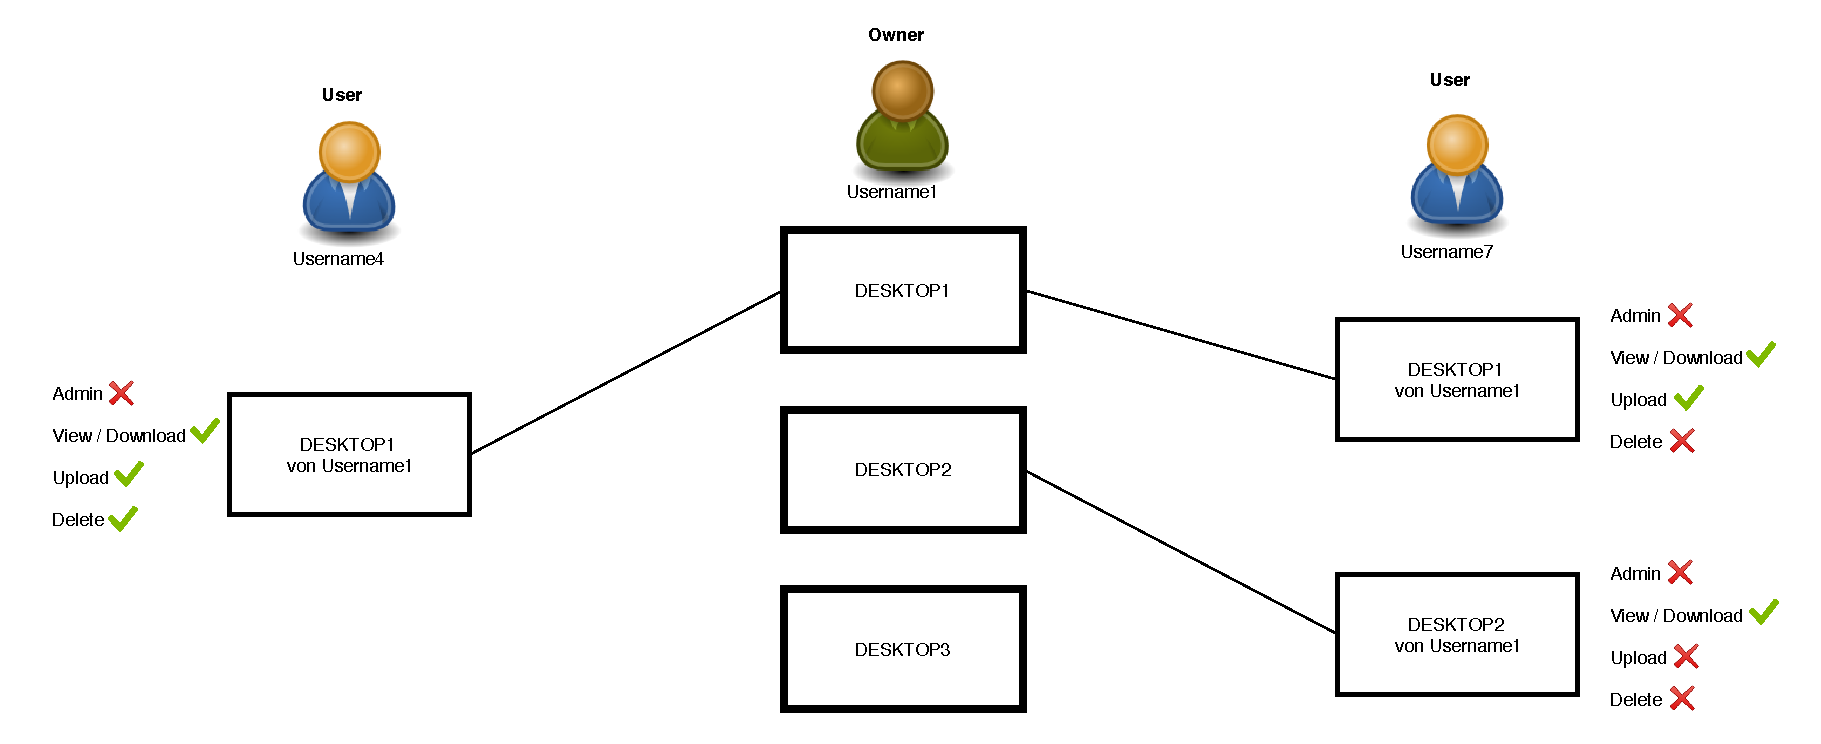
\includegraphics[scale=0.45]{VD_konzept.pdf}
\caption{Username1 ist Owner und besitzt drei Desktops. DESKTOP1 teilt Username1 mit Username4 und Username7. Der DESKTOP2 wird nur mit Username7 geteilt. Den Usern wurden individuell für diese Desktops Rechte zugeteilt. Den DESKTOP3 kann nur der Owner selbst betrachten.}
\end{figure}

\noindent Ein Anwender, der nicht explizit jedem mit dem er seinen Desktop zu teilen vermag, Rechte zuweisen möchte, weil es sich z.B. um eine sehr große Anzahl von Personen handelt, kann als \textit{Owner} seinen Desktop auf public setzen.
Da Desktopnamen in \textit{VirtualDesktop} global eindeutig sind, kann dieser Desktop dann über den Desktopnamen geteilt und gefunden werden.
\textit{User} haben auf einem, auf public gesetzten, Desktop nur Leserechte, außer ihnen wurden explizit weitere Rechte zugewiesen. 
Nur dem \textit{Owner} ist es erlaubt den Desktop wieder auf privat zu setzen, auch \textit{Usern} mit Admin-Rechten für diesen Desktop ist dies nicht gestattet.

\chapter{Der Weg in die Cloud}
% todo klassiche web projekt beschreiben. probem mit max gleichzeitiger verbindungen. bild von vorlesung beschreiben. dran denken an wins. lieber kontrole abgeben mehr enwickeln. nodejs = geschätslogik
(dadurch wird die skalierung schonmal besser)

Es gibt verschiedene Wege, wie man eine Web-Applikation aufsetzt. Die ersten Schritte wird man meist auf einer lokalen Entwicklungsumgebung machen, die man auch zum späteren entwickeln braucht. Irgendwann wird man sich aber die Frage stellen, wo die spätere Infrastruktur laufen wird. \\
Der Weg in die Cloud benötigt zu Beginn einen entscheidenden Schritt. Man muss sich für einen Cloudanbieter entscheiden. Es gibt verschiedenste Anbieter wie GoogleCloud von Google, AWS von Amazon oder Azure von Microsoft. \\
Im Rahmen des Moduls CloudComputung an der HS-RM haben wir uns dazu entschlossen die Cloud Services von AWS - Amazon zu nutzen.
\section{Warum geht man in die Cloud}
asd
\section{Anforderungen an die Skalierbarkeit}
Unsere Projektanforderungen an die Architektur umfasst einen klassischen Aufbau eines Web Projektes mit folgenden Anforderungen. \\

\begin{itemize}
\item Eine Laufumgebung auf der NodeJS läuft.
\item Eine Datenbank, die auch mit vielen Zugriffen schnell bleibt.
\item Einen Speicher, der die Daten von den Nutzern speichert.
\item Alle Zugriffe müssen authentifiziert werden.
\item Skalierung soll jederzeit möglich sein, um beliebig viele Nutzer bedienen zu können.
\end{itemize}
Es wäre durchaus denkbar die ersten vier Punkte gut auf einer klassischen, nicht Cloudservice basierenden Serverumgebung umzusetzen. Aber spätestens bei der beliebigen Skalierung stößt man auf Probleme. 
\\
Die auf einer klassischen Serverumgebung einfach mögliche vertikale Skalierung stößt schnell auf ihre Grenzen. Früher oder später wird vermutlich die Datenbank in jedem System der Flaschenhals werden und diese dann horizontal zu skalieren ist meist mit großen strukturellen und/oder architektonischen Änderungen verbunden.

\section{Vorteile Infrastruktur}
%dieser satz eher am anfang. villeicht ganze kapitel.
Eine Umsetzung in AWS bringt ein Umdenken mit sich. In AWS wird jeder Service in eigenen Teil gesplittet. Rechner, Speicher, Datenbank, Authentifizierung, Domainverwaltung sogar einzelne Funktionen liegen einzeln in AWS vor. Dadurch ist eine unabhängige Skalierung überhaupt möglich. \\
%todo umschreiben wir müssen schon kümmern = mappen
Um das Projekt umzusetzen brauchen wir uns dank der Cloudservices nicht um Dinge, wie den NodsJS Server, den Speicher, die Virtualisierung oder das Netzwerk kümmern. \\
Auch um die Laufzeitumgebung und um das Betriebssystem brauchen wir uns nicht kümmern. Wir legen sie lediglich fest. Dank der Cloudservices von AWS können wir uns nach dem Aufsetzen und Verknüpfen aller unser genutzten Service ganz auf die Programmierung konzentrieren.
\section{Vorteile Skalierung}
%vermutlich kann weg
Das Hauptproblem von Anwendungen, die erfolgreich von vielen Nutzern genutzt wird ist die Skalierung.
\subsection{Skalierung Plattform / Laufzeitumgebung}
%todo Leastic Beasntalk geht gerade auf klassische webprojekte ab. Alle alten webanwendungen könnte man dort abbilden. (PHP, java ..). Das ist der erste Punkt. Wenn man noch verweden möchte einfach das. mit zunehmen kenntnissen voll auf aws diensten umsteigen dann ressourcen auslagern etc
Auf unserer Laufzeitumgebung läuft ein NodeJS Server. Dieser wird durch Elastic-Beanstalk automatisch skaliert. Die Rechenleistung also die CPU, der Arbeitsspeicher wie der interne genutzte Speicher wird dynamisch je nach Bedarf angepasst. \\
Eine klassische Umsetzung auf einen Server kann man lediglich vertikal skalieren und den Arbeitsspeicher oder die CPU aufrüsten. 
\subsection{Skalierung Speicher und Datenbank}
Der Speicher wird bei AWS klassischerweise mit S3 umgesetzt. Der S3 Speicher hat eine Skalierung inkludiert. \\
%todo umschreiben nicht sprechend. Typisch über SQL reden.
Es gibt verschiedenste Datenbanktypen, die meisten sind nur schwer skalierbar. AWS bietet die DynamoDB an um Dokumente mit Schlüsselwerten zu speichern. DynamoDB skaliert ebenfalls automatisch. Die globalen DynamoDB Tabellen replizieren sich automatisch über mehrere AWS-Regionen \cite{AWSa}.\\
%QUELLE DYNAMODB
%https://aws.amazon.com/de/dynamodb/
\subsection{Skalierung Netzwerk}
Auch um den Datendurchsatz bei der Netzwerkübertragung  braucht man sich dank verteilter Rechenzentren, die sich je nach Nutzungsort verändern können nicht zu kümmern. Plant man einen internationalen Einsatz ist ein Einsatz von Amazon CloudFront / CDN erweiterbar \cite{AWSb}.%QUELLE CLOUDFRONT
%https://aws.amazon.com/de/cloudfront/
\section{Sicherheit}
Anstatt sich händisch darum zu kümmern sein System aktuell bleibt, kann man bei Cloudservices auf die Expertise von Profis zurückgreifen. Updates und Sicherheitspatches werden automatisch eingespielt, über Firewall und Antiviren Programme braucht man sich keine Sorgen mehr machen. \\
Außerdem nimmt AWS mit verschiedenen Services Sicherheitsimplementierungen ab. Cognito ermöglicht schnell und einfach eine Double Opt in Registrierung umzusetzen.
\section{Kosten}
%vom Monolith weg - hoch schieben man zahlt nur das was man verbraucht
Die Skalierung klassischer Webprojekte läuft so, dass die Infrastruktur für die maximale Nutzung aufgebaut wird. Das bedeutet, dass bei hoher kurzzeitiger Nutzung Ressourcen aufgebaut werden, die dann kurz danach nicht mehr benötigt werden. Ein Rückbau wird selten gemacht und Ressourcen liegen brach.\\
Dieses überpowern der Infrastruktur birgt vermeidbare Mehrkosten. AWS rechnet immer nur den aktuellen Verbrauch ab. Wird ein Server Nachts nicht genutzt, werden keine Kosten generiert. Alle zusätzlichen Kosten einer klassischen Infrastruktur wie Wartung, sind darin bereits inkludiert.
\section{Was gibt es für Cloudanbieter}

\section{CloudLockin}
%todo CloudLockin gerade auf datenbank dynamoDB!
%erster Abschnitt hierrein

\chapter{Architektur}
% Clouformation ansprechen
% Hier wie deploye ich rein
Um in AWS seinen Service Stack zu persistieren haben wir \textit{Clouformation} genutzt. In \textit{Cloudformation} wird anhand einer template Datei der Stack in yml oder json beschrieben. \\
Wie bereits in den Anforderungen beschrieben, haben wir uns als Ziel gesetzt den gesamten Service Stack mit einen Befehl ausrollen zu können. Der Befehl mit den Parametern wird im setup Ordner ausgeführt und ist folgender:

\begin{lstlisting}[xleftmargin=\parindent,frame=L,mathescape=true, basicstyle=\small, language=Java, lineskip={1.0pt}]
node index.js create <aws_key_id> <aws_access_key> 
<stack_name> [<domainName>]
\end{lstlisting}

Die Voraussetzung, um unser Stack Deployment Script ausführen zu können ist die Installation von node und aws-cli und ein anschließendes npm install.
Mit der Ausführung des Scripts werden die Lambda und unsere Anwendung inklusive der benötigten Dateien in einen \textit{CodeBucket} hochgeladen, womit in \textit{Cloudformation} dann die Anwendungen aufgebaut werden. Ein Abbau des Stacks ist ebenso möglich.

\begin{lstlisting}[xleftmargin=\parindent,frame=L,mathescape=true, basicstyle=\small, language=Java, lineskip={1.0pt}]
node index.js delete <aws_key_id> <aws_access_key>
 <tmp_code_bucket_name> <stack_name>
\end{lstlisting}

Dieser Aufruf wird nach dem ausführen des deployment Scripts mit den bereits ausgefüllten Parametern ausgegeben. \\
Die daraus entstehende Servicearchtitektur kann man in folgender Grafik zusammenfassen.

\begin{figure}[h!]
\centering
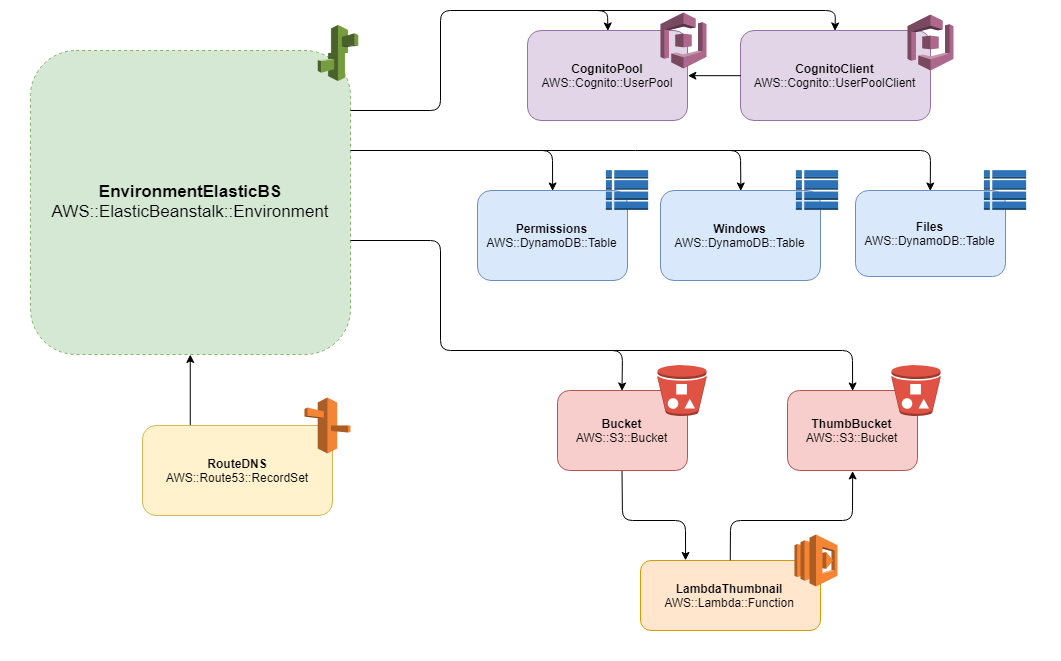
\includegraphics[scale=0.45]{ArchiDiagram.png} 
\caption{Architekturdiagramm Virtual-Desktop}
\end{figure}

Im folgenden Kapitel werden die einzelnen Services und deren Konfiguration in \textit{Cloudformation} beschrieben. 

\newpage
\section{Elastic Beanstalk Konfiguration}
Die Geschäftslogik wird in unserer EC2 Instanz abgewickelt, welcher in ein ElasticBeanstalk Stack skaliert wird. Dieser Stack sorgt dafür, dass die EC2 Instanz im Speicher, in der Rechenleistung, im Netzwerk wie auch im Arbeitsspeicher je nach den derzeitiger Anforderung skaliert. Wie man in der Grafik sehen kann, braucht eine Elastic-Beanstalk Applikation auch immer ein Elastic-Beanstalk Umgebung und ein Konfigurationstemplate. In Auszügen zeige ich die ElasticBeanstalk Konfiguration.

\begin{lstlisting}[xleftmargin=\parindent,numbers=left,numberstyle=\small,numbersep=8pt,frame=L,mathescape=true, basicstyle=\small, language=Java, lineskip={1.0pt}]
ElasticBS:
        Type: AWS::ElasticBeanstalk::Application
        Properties:
            Description: ElasticBeanstalk VirtualDesktop
    ApplicationVersionElasticBS:
        Type: AWS::ElasticBeanstalk::ApplicationVersion
        Properties:
            ApplicationName:
                Ref: ElasticBS
            Description: ElasticBeanstalk VirtualDesktop
             Application Version
            SourceBundle:
                S3Bucket:
                    Ref: CodeBucket
                S3Key: ebs.zip
\end{lstlisting}
Interessant ist hier die ElasticBeanstalk Appplikation zugrunde liegende Code, der in einen seperaten CodeBucket als zip vorliegt. Von dort aus wird die Applikation in der EC2 Instanz gebaut.
Die ElasticBeanstalk Umgebung
 \textit{AWS::ElasticBeanstalk::Environment} beinhaltet die Konfiguration der eigentlichen Instanz.
\begin{lstlisting}[xleftmargin=\parindent,numbers=left,numberstyle=\small,numbersep=8pt,frame=L,mathescape=true, basicstyle=\small, language=Java, lineskip={1.0pt}]
    EnvironmentElasticBS:
        Type: AWS::ElasticBeanstalk::Environment
        Properties:
            ApplicationName:
                Ref: ElasticBS
            Description: AWS ElasticBeanstalk VirtualDesktop 
            Environment
            TemplateName:
                Ref: ConfigurationElasticBS
            VersionLabel:
                Ref: ApplicationVersionElasticBS
            OptionSettings:
            -
                Namespace: aws:autoscaling:launchconfiguration 
                OptionName: IamInstanceProfile
                Value: aws-elasticbeanstalk-ec2-role
            -
                Namespace: aws:elasticbeanstalk:container:nodejs
                OptionName: NodeCommand
                Value: "npm start"
\end{lstlisting}

Dort werden zum Beispiel die Laufzeit und die Umgebungsvariablen über die ElasticBeanstalk Konfiguration festgelegt. Auch den Start Befehl beim hochfahren der Instanz kann man dort festlegen.\\
ElasticBeanstalk legt neben den hier beschriebenen Services auch Services an, die nicht explizit konfiguriert werden, wie einen \textit{LoadBalancer}, \textit{CloudWatch} und verschiedenste Berechtigungen. Dies benötigt ElasticBeanstalk, um die automatische Skalierung überhaupt möglich zu machen. \\
Die EC2 Instanz beinhaltet unsere NodeJS Applikation und stellt sowohl das Front- wie Backend. Mit einer API werden dort die Operationen auf den AWS-Services koordiniert und gesteuert. 
%todo Configuration Template mit rein nehmen und beschreiben (nur einen Key zeigen)

\section{Authentifizierungsservice Cognito}
%Inhaltlich gut
Zur Authentifizierung von Nutzern wird der AWS Cognito verwendet. Der Nutzerpool \textit{Cognitopool} vom Typ \textit{AWS::Cognito::UserPool} ist so konfiguriert, dass bei der Registrierung eines neuen Nutzers ein Passwort angegeben werden muss, welches die Minimalvorrausetzung eines AWS-Cognito-Passworts erfüllt (Zeichenlänge von Sechs \cite{AWSD}). Für die Registriereung muss der Nutzer sich verifizieren. Dies geschieht hier über Email, in der der Nutzer seinen Bestätigungscode erhält. Die Formatierung dieser Email wird in \textit{EmailVerificationMessage} und \textit{EmailVerificationSubject} angegeben.  
%COGNITO MINLÄNGE
%https://docs.aws.amazon.com/de_de/AWSCloudFormation/latest/UserGuide/aws-properties-cognito-userpool-passwordpolicy.html
\begin{lstlisting}[xleftmargin=\parindent,numbers=left,numberstyle=\small,numbersep=8pt,frame=L,mathescape=true, basicstyle=\small, language=Java, lineskip={1.0pt}]
CognitoPool:
        Type: AWS::Cognito::UserPool
        Properties:
            AutoVerifiedAttributes:
                -
                    "email"
            EmailVerificationMessage: "Here is your code: {####}"
            EmailVerificationSubject: "Verify your E-Mail for VD"
            Policies:
                PasswordPolicy:
                    MinimumLength: "6"
                    RequireLowercase: false
                    RequireNumbers: false
                    RequireSymbols: false
                    RequireUppercase: false

\end{lstlisting}
\bigskip
\noindent Um den \textit{UserPool} verwenden zu können, benötigt dieser einen Benutzer, den \textit{AWS::Cognito::UserPoolClient}. Dieser wird über die Property \textit{UserPoolId} an den angegeben \textit{UserPool} gebunden, in diesem Fall wird eine Referenz auf den zuvor angelegten UserPool mit dem Namen \textit{CognitoPool} angegeben. Die Property \textit{GenerateSecret} wird hier auf \textit{false} gesetzt, da die clientseitig verwendete Amazon Cognito Identity-SDK für JavaScript keine client secrets unterstützt \cite{AWSAmplify}.
%generateSec QUelle
%https://github.com/aws-amplify/amplify-js/tree/master/packages/amazon-cognito-identity-js

\begin{lstlisting}[xleftmargin=\parindent,numbers=left,numberstyle=\small,numbersep=8pt,frame=L,mathescape=true, basicstyle=\small, language=Java, lineskip={1.0pt}]
    CognitoClient:
        Type: AWS::Cognito::UserPoolClient
        Properties:
            GenerateSecret: false
            UserPoolId: '{"Ref" : "CognitoPool"}'
\end{lstlisting} 

\section{Cloud-Speicher S3}
Unsere Applikation benötigt insgesamt 3\textit{ S3- Buckets.} Der erste Bucket, auch später \textit{Code Bucket} genannt, wird nur temporär während des Aufbaus des Stacks benötigt. Cloudformation setzt die gezippte Anwendung inklusive Template Definition beim Aufbau voraus. Dieser Bucket wird beim entfernen des Stacks mit dem Deployment Script wieder gelöscht. \\
Ein weiterer Bucket wird gebraucht, um die Daten der Nutzer zu speichern. Dort liegen ausschließlich die Nutzermediendaten. Dieser Bucket wird im folgenden User Bucket genannt. \\
Zuletzt wird ein weiterer Bucket genutzt, um die Thumbnails der Bilder, die durch unseren LambdaService generiert werden, zu speichern. Der Thumbnail Bucket, hat ein Präfix \textit{thumbs} und sonst denselben generischen Namen wie der User Bucket. \\
Durch folgende Beschreibung in der Konfiguration wird der Thumbnail Bucket erstellt.
\begin{lstlisting}[xleftmargin=\parindent,numbers=left,numberstyle=\small,numbersep=8pt,frame=L,mathescape=true, basicstyle=\small, language=Java, lineskip={1.0pt}]
ThumbBucket:
    Type: AWS::S3::Bucket
    Properties:
        BucketName: !Sub
            - thumbs{ResBucket}
            - ResBucket: !Ref Bucket
\end{lstlisting}          
Auch die S3-Buckets haben in AWS eine automatische Skalierung inne. Sowohl in der Größe, wie auch in der genutzten Bandbreite ist der Speicher variabel und passt sich den Umständen an.

\section{Datenbank DynamoDB}
Aufgrund der Architektur der Applikation und der Festlegung die Infrastruktur in der Cloud laufen zu lassen, kam für uns nur eine NOSQL Datenbank wie DynamoDB in Frage. Eine SQL Datenbank, wäre für unseren Einsatz zwar möglich, würde aber nur zusätzliche Komplexität und Einschränkungen mit sich bringen. \\
Das Erstellung einer Datenbanktabelle in der DynamoDB wird hier exemplarisch an der \textit{Permissions}-Tabelle vom Typ \textit{AWS::DynamoDB::Table} gezeigt. Anders als bei klassischen SQL-Datenbanken kann ein Eintrag in einer DynamoDB-Tabelle beliebige Felder beinhalten. Diese werden lediglich über den Schlüssel abgefragt. Um den Schlüssel einer Tabelle zu definieren muss der \textit{AttributeType}, der \textit{AttributeName} und der \textit{KeyType} innerhalb der \textit{AttributeDefinitions} und \textit{KeySchema} angegeben werden. Diese beiden Felder sind erforderlich, müssen also angegeben werden. Das selbe gilt für \textit{ProvisionedThroughput} \cite{AWSDa}.
Dies bedeutet, dass die Skalierung nicht bei der Erstellung durch CloudFormation oder EBS eingestellt werden werden. Um die DynamoDB zu skalieren muss \textit{AWSServiceRoleForApplicationAutoScaling\_DynamoDBTable} im AWS-Account aktiv sein. Falls \textit{AWSServiceRoleForApplicationAutoScaling\_DynamoDBTable} bereits bei der Erstellung durch EB-Deploy aktiviert war skalieren die Tabellen,  ansonsten nicht. Das Autoscaling für die Tabellen kann dann jedoch nachträglich über die Management-Console eingestellt werden. Nähere Informationen hierzu sind in \cite{AWSDb} zu finden.
\\

%- Was ist das Problem. Nicht mehrere Sachen löschen nicht möglich.
Da die DynamoDB nicht über die Möglichkeit verfügt, mehrere Einträge über einen Key zu entfernen, muss für die \textit{deleteWindow}-Funktion die gesamte \textit{File}-Liste und \textit{Permission}-Liste für den gegebenen Key eingelesen und jeder Eintrag einzeln in der DynamoDB entfernt werden.
Um nicht jeden Listeneintrag einzeln zu entfernen kann zwar \textit{batchWriteItem} verwendet werden, dieses ist jedoch max. auf 25 DeleteItem-Operationen limitiert und es können keine \textit{conditions} angegeben werden \cite{AWSJSSDKD}. Aus diesem Grund werden die Items, wie hier einleitend erwähnt, einzeln entfernt.

%deleteITEM AWS
%https://docs.aws.amazon.com/AWSJavaScriptSDK/latest/AWS/DynamoDB.html#deleteItem-property

%QUELLE allg.DYNDB
%https://docs.aws.amazon.com/de_de/AWSCloudFormation/latest/UserGuide/aws-resource-dynamodb-table.html


%QUELLE AUTOSCALING
%https://docs.aws.amazon.com/de_de/amazondynamodb/latest/developerguide/AutoScaling.Console.html


\begin{lstlisting}[xleftmargin=\parindent,numbers=left,numberstyle=\small,numbersep=8pt,frame=L,mathescape=true, basicstyle=\small, language=Java, lineskip={1.0pt}]
Permissions:
        Type: AWS::DynamoDB::Table
        Properties:
            AttributeDefinitions:
                -
                    AttributeName: "Window"
                    AttributeType: "S"
                -
                    AttributeName: "User"
                    AttributeType: "S"
            KeySchema:
                -
                    AttributeName: "Window"
                    KeyType: "HASH"
                -
                    AttributeName: "User"
                    KeyType: "RANGE"
            ProvisionedThroughput:
                ReadCapacityUnits: "1"
                WriteCapacityUnits: "1"
\end{lstlisting}

Unsere Applikation benötigt 3 Tabellen. Eine Tabelle \textit{Files} speichert die Relation zwischen \textit{FileName}, \textit{WindowName} und \textit{User}. So kann man den jeweiligen Desktops die Dateien zuordnen, und auch die Besitzer der Dateien herausfinden. In der zweiten Tabelle \textit{Windows} werden der Desktop Namen \textit{WindowName}, der Besitzer \textit{Owner} und ein Flag ob der Desktop pubic ist oder nicht gespeichert.Die dritte Tabelle \textit{Permissions} ordnet den Desktops die Berechtigungen einzelner Nutzer zu. Die Spalten lautet hier \textit{Window}, \textit{User}. \textit{Permissions}. Die Permissions der einzelnen Nutzer werden als JSON gespeichert und beinhalten Informationen über das Recht Admin zu sein, lesen, schreiben oder löschen zu dürfen, auf den jeweiligen Desktop. \\
In der Applikation wird bei jeder Operation überprüft ob der jeweilige Nutzer die Berechtigung hat dies zu tun.

\section{Serverless-Functions Lambda}
Der FaaS Dienst Lambda wird in unserer Applikation genutzt, um unabhängig von unserer EC2 Instanz die Vorschaubilder bzw. Thumbnails für die Bilder, die die Nutzer hochladen zu generieren. Der Vorteil von Lambda ist, dass man sich nicht um die Laufzeitumgebung kümmern muss und das man keine EC2 Instanz ständig laufen lassen muss, damit eine NodeJS Funktion eventbasierend ausgeführt wird. \\ 
Bei der Konfiguration von Lambda in \textit{Cloudformation} müssen mehrere Ressourcen beachtet werden. \\
Unsere Lambda Funktion benötigt eine Rolle, die sowohl \textit{Permissions} wie \textit{Policies} hält. Die Rolle braucht die Erlaubnis Lambda Funktionen aufzurufen, wenn etwas in unseren \textit{UserBucket} hochgeladen wird. Dies wird folgendermaßen konfiguriert:

\begin{lstlisting}[xleftmargin=\parindent,numbers=left,numberstyle=\small,numbersep=8pt,frame=L,mathescape=true, basicstyle=\small, language=Java, lineskip={1.0pt}]
LambdaPermission:
    Type: "AWS::Lambda::Permission"
    Properties: 
        Action: "lambda:InvokeFunction"
        FunctionName:
            Fn::GetAtt:
            - LambdaThumbnail
            - Arn
        Principal: "s3.amazonaws.com"
\end{lstlisting}

Außerdem wird eine Policy erstellt, um Logs und S3 Objekte zu schreiben und XRAYs verfolgen zu können.\\
Die Lambda Funktion benutzt dann diese Rolle, um alle Dinge zu bewerkstelligen die wir für das erstellen der Thumbnails benötigen. Die Lambda Funktion wird folgendermaßen konfiguriert:

\begin{lstlisting}[xleftmargin=\parindent,numbers=left,numberstyle=\small,numbersep=8pt,frame=L,mathescape=true, basicstyle=\small, language=Java, lineskip={1.0pt}]
LambdaThumbnail:
    Type: "AWS::Lambda::Function"
    Properties: 
        Handler: "index.handler"
        Role: 
            Fn::GetAtt: 
                - "LambdaRole"
                - "Arn"
        Code:
            S3Bucket:
                Ref: CodeBucket
            S3Key: "lambda.zip"
        MemorySize: "1024"
        Runtime: "nodejs8.10"
        Timeout: "10"
        TracingConfig:
            Mode: "Active"
\end{lstlisting}

Wie man sieht gibt man in Zeile 3 den Einstiegspunkt mit, benutzt in den folgenden Zeilen die definierte Rolle und greift auf den gezippten Quellcode im definierten CodeBucket zu. Die restlichen Zeilen geben die Parameter für die Laufzeitumgebung an, wie die Arbeitsspeichergröße, den Funktionsname, die Laufzeit, Timeout und das erlaube XRAY Tracing.\\

Die Funktion wird durch ein S3 \textit{s3:ObjectCreated:*} Event gestartet. Das Thumbnail Script filtert zuerst die Bilder aus den Anfragen, anhand der Dateiendungen heraus. Diese Bilder werden daraufhin verkleinert und in einen zweiten Bucket mit denselben Namen hochgeladen. Dieser zweite Bucket hat denselben Namen wie der Ursprungsbucket mit dem Präfix \textit{thumbs}. Damit kann man nun einfach aus dem NodeJS System auf das Thumbnail zugreifen. \\
Ist das Thumbnail nicht vorhanden, wird ein generisches Vorschaubild erzeugt. 
\subsection{XRAY}
Wer eine Lambda Funktion über Cloudformation definiert und hochfährt wird unweigerlich über XRAY stolpern. Mit einer Fehlermeldung wie: 
\begin{lstlisting}
The provided execution role does not have permissions to
call PutTraceSegments on XRAY
\end{lstlisting}
wird die Erstellung abgebrochen. Wird eine Lambda Funktion durch ein Service wie Cloudformation getriggert, braucht Lambda keine weiteren Berechtigungen, da Lambda diese in den Stack-Kontext bereits besitzt. Unser Lambda Service wird aber durch ein Event getriggert. Wenn ein User etwas in den Userbucket lädt, wird die Lambda Funktion ausgeführt. Dadurch fehlt der Funktion der Stack Kontext, auch wenn er durch jenen erstellt wurde. \\
Seit Anfang 2018 \cite{AWSDe} ist es möglich durch hinzufügen von
\begin{lstlisting}
Properties:
  TracingConfig:
    Mode: "Active"
\end{lstlisting} 
in dem Service \textit{AWS::Lambda::Function} und mit 
\begin{lstlisting}
Properties:
  PolicyDocument:
  -
    Effect: Allow
    Action:
    - xray:PutTraceSegments
    - xray:PutTelemetryRecords
    Resource: '*'
\end{lstlisting} 
in dem Lambda Funktion genutzte Policy \textit{AWS::IAM::Policy}
%QUELLE XRAY
%https://docs.aws.amazon.com/de_de/xray/latest/devguide/xray-services-lambda.html

\section{Route53}
Um die generierte ElasticBeanstalk Domain auf eine sprechender Domain zu mappen, in unserem Fall \textit{www.virtual-desktop.org}, nutzen wir den Route53 Service. Die Konfiguration setzt eine registrierte Route53 Domain bei AWS voraus:

\begin{lstlisting}[xleftmargin=\parindent,numbers=left,numberstyle=\small,numbersep=8pt,frame=L,mathescape=true, basicstyle=\small, language=Java, lineskip={1.0pt}]
RouteDNS:
    Type: AWS::Route53::RecordSet
    Properties:
        HostedZoneName: !Sub
            - ${DName}.
            - DName: !Ref DomainName
        Name: !Sub
            - www.${DName}.
            - DName: !Ref DomainName
        Type: CNAME
        TTL: 900
        ResourceRecords:
        - !GetAtt EnvironmentElasticBS.EndpointURL
\end{lstlisting}

Der Domain Name wird per Startparameter von den Cloudformation Start-Script gesetzt. Per \textit{ResourceRecords} wird die ElasticBeanstalk Domain gesetzt.
 
\section{Wie arbeiten die Services zusammen}

Um das zusammenarbeiten der einzelnen Services zu demonstrieren, zeigen wir beispielhaft verschiedene Szenarien. Wir gehen in den einzelnen Szenarien unterschiedlich detailliert, auf die genutzten Dienste ein, um den Fokus nach unseren Wünschen zu setzen:
\begin{itemize}
\item Ein Nutzer logt sich mit einen Username und Passwort ein.
\item Ein Nutzer lädt ein Bild hoch.
\end{itemize}

\begin{figure}[h]
\centering
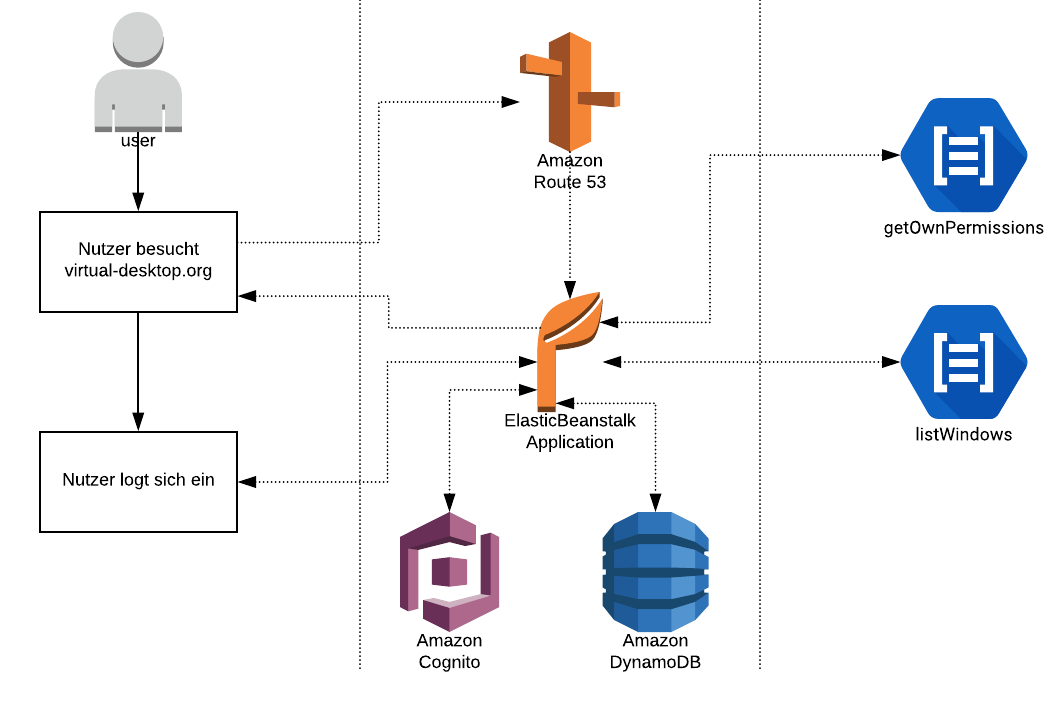
\includegraphics[scale=0.35]{Flow-Dia-1.png} 
\caption{User logt sich ein}
\end{figure}

Zeitlich gesehen ist der erste AWS Service, den man als Anwender nutzt der Route53 Service, der für das Routing der Domain \textit{www.virtual-desktop.org} auf die ElasticBeanstalk Domain zuständig ist. Daraufhin wird das Frontend von der EC2 Instanz dem Nutzer geliefert. Logt der Nutzer sich ein, wird von der Applikation mit Hilfe des \textit{Cognito} Services, der jeweilige Nutzer authentifiziert. Ist die Authentifizierung erfolgreich, wird in der DynamoDB über die API die Berechtigungen und die Desktops, die der Nutzer sehen darf abgefragt. Der Nutzer bekommt daraufhin die benötigten Daten in das Frontend gerendert und sieht alle Desktops auf die er Zugriff hat. \\

\begin{figure}[h]
\centering
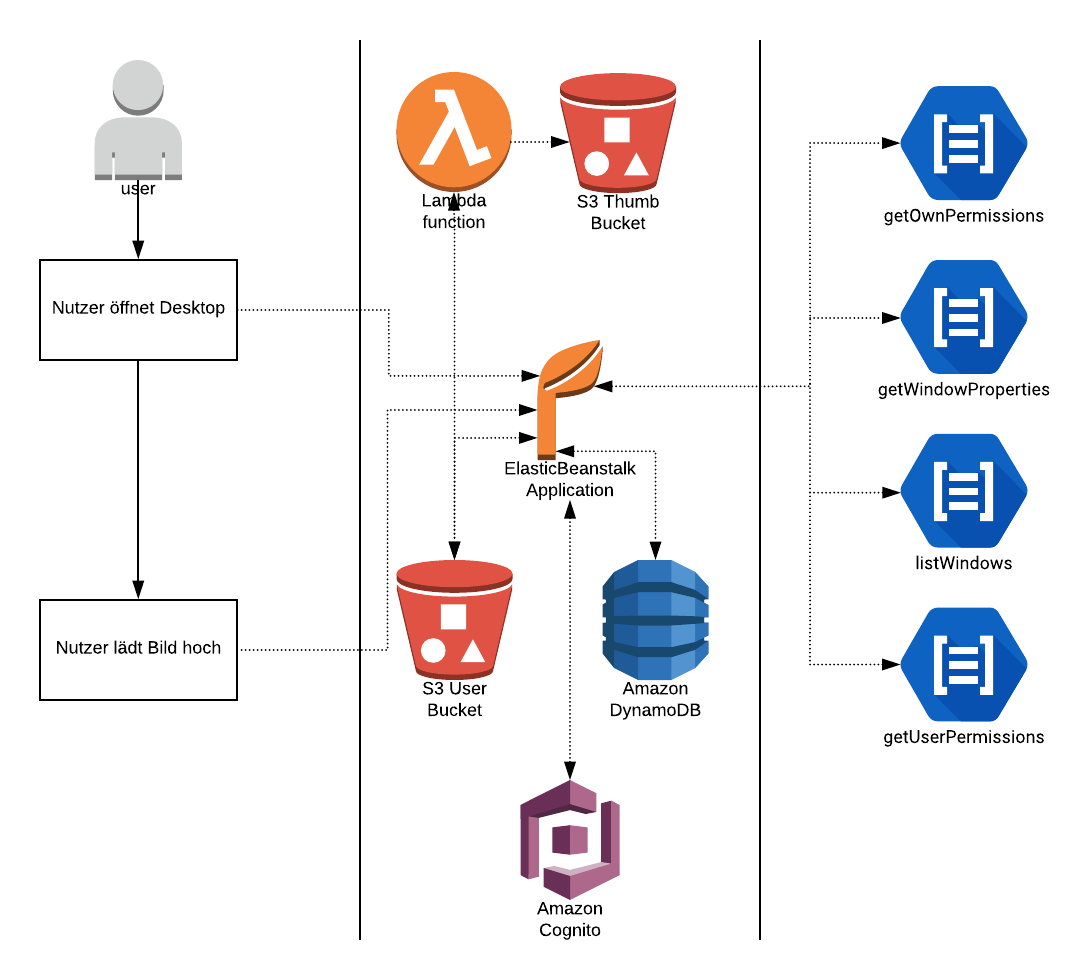
\includegraphics[scale=0.6]{Flow-Dia-12.png}
\caption{User läd ein Bild hoch}
\end{figure}

Das zweite Szenario beschreibt das hochladen eines Bildes auf einen Desktop. Lädt der Nutzer eine Datei in einen Desktop wird zuerst überprüft, ob er überhaupt Schreibberechtigung hat. Ist dies der Fall wird das Bild als Stream über die EC2 Instanz in den User Bucket hochgeladen. Der große Vorteil des Streams ist, dass die Datei nicht zuerst komplett in die EC2 Instanz geladen wird und von dort aus in den User Bucket geladen wird, sondern immer nur ein kleiner Teil in der EC2 Instanz liegt bevor die Datei in den User Bucket gelegt wird. Während des Uploadvorgangs bekommt der Nutzer ein Feedback, dass der Upload noch andauert. Sobald die Datei komplett auf dem S3 angekommen ist, sieht der Nutzer das Bild in den Desktop. Wird eine Datei mit der Endung \textit{jpg, jpeg oder png} in den User Bucket erstellt, wird durch ein S3 Event der Thumbnail Lambda Service gestartet und das Thumbnail wird in den \textit{thums} Bucket abgelegt. Besucht ein Nutzer nun das nächste Mal diesen Desktop sieht er das Bild mit Thumbnail auf dem Desktop.



\chapter{Besonderheiten}
Im folgenden beleuchten wir möglichst kurz die unser Meinung nach interessanten Stellen der Umsetzung der Applikation.

\section{Entwicklungsumgebung lokal / Env- Variablen in NodeJS}
%- Refs lösen

Bei Elastic-Beanstalk-Projekten wird bei jedem Deploy die gesamte Umgebung mit allen AWS-Resourcen neu gestartet. Dies beinhaltet unter anderem die EC2-Instanz. Da bei Quellcodeänderungen ein Deploy erneut ausgeführt werden muss und die Instanziierung einer EC2-Instanz zeitaufwendig sein kann ist dies für die Entwicklung der Webanwendung nicht praktikabel. Aus diesem Grund wurden in Elastic-Beanstalk, Referenzen \cite{AWSDc} für die dynamisch angelegten Ressourcen erzeugt. Diese Referenzen können in Umgebungsvariablen der EC2-Instanzen übernommen werden, dies geschieht in der \textit{node-env-keys.config} \cite{AWSDd}.\\
Um eine schnellere Entwicklung voranzutreiben wird dieser Umstand genutzt, indem statische (nicht durch EBS-Deploy generiert) Amazon Web Services erstellt und in die Umgebungsvariablen des Entwicklersystems hinzugefügt werden.
Hierbei ist zu beachten, dass lediglich die EC2-Instanzen durch den lokalen Rechner ersetzt werden. Anzulegende Umgebungsvariablen sind
\textit{AWS\_ACCESS\_KEY\_ID} und \textit{AWS\_SECRET\_ACCESS\_KEY} mit den AWS-Credentials, \textit{COGNITO\_CLIENT} und \textit{COGNITO\_POOL} mit der App-Client-ID eines Cognito-Clients (mit GenerateSecret=false) und der Pool-ID des dazugehörigen Cognito-Pools, \textit{FILES}, \textit{PERMISSIONS} und \textit{WINDOWS} mit den jeweiligen Tabellennamen von DynamoDB-Tabellen mit der Struktur beschrieben in [.\textbf{TODO}.] und \textit{BUCKET} sowie \textit{THUMB\_BUCKET} mit den Bucket-Namen. Weiterhin muss die Lambda-Funktion wie in \textbf{LAMDBA TODO} beschrieben  für die Generierung von Thumbnails erstellt werden. Die Lambda-Funktion muss mit den Buckets verknüpft sein.  


%REF QUELLE
%https://docs.aws.amazon.com/de_de/AWSCloudFormation/latest/UserGuide/intrinsic-function-reference-ref.html

%EVI VAR
%https://docs.aws.amazon.com/de_de/elasticbeanstalk/latest/dg/environments-cfg-softwaresettings.html


\section{Promise / Dispatcher}
%ok

Die Funktion der AWS-sdk arbeiten mit Callbacks, jedoch sind Aufgaben wie z.B. das Löschen von Desktops und deren Inhalt parallelisierbar, und müssen synchronisiert werden. Um dies zu bewerkstelligen, und um komplexe Callbackstrukturen zu vermeiden wurde eine \textit{dispatch}-Funktion für solche Aufgaben konzipiert. 

\begin{lstlisting}[xleftmargin=\parindent,numbers=left,numberstyle=\small,numbersep=8pt,frame=L,mathescape=true, basicstyle=\small, language=Java, lineskip={1.0pt}]
async function dispatch(tasks, map, callback) {
    var data = { tasks: tasks,
                 map: map, 
                 result: {}, 
                 errors: [], 
                 propergate: true 
    };
    while(data.tasks.length != 0 && data.propergate) {
        var promises = [];
        for (var i = 0; i < tasks[0].length; i++) {
            var f = function(resolve, reject) {
                    this.tasks[0][i](this, () => {
                    resolve();
                });
            };
            promises.push(new Promise(f.bind(data)))
        }
        await Promise.all(promises);
        data.tasks.splice(0, 1);
    }
    callback(data);
}
\end{lstlisting}

Es wird hier zum einen der Parameter \textit{tasks}, einem Array aus Arrays aus Funktionen, der Form \textit{(dis, done)}, sowie ein Objekt \textit{map}, welches innerhalb der \textit{tasks} über \textit{dis.map} zugreifbar ist, und einer \textit{callback}-Funktion, welche nach Beendigung aller \textit{tasks} ausgeführt und die Resultate und Fehler zurückliefert, übergeben. Der \textit{callback} ist notwendig, da die Funktion asynchron ist. Die \textit{dispatch}-Funktion sorgt dafür, dass die Funktionen der inneren \textit{task}-Arrays parallel durch die Kapselung in \textit{promisses} ausgeführt werden. Der Array selbst wird sequentiell ausgeführt, dies wird durch \textit{await} sichergestellt. Es ist zu dem möglich, während des \textit{dispatch}-Prozesses weitere \textit{tasks} hinzuzufügen (dies wird z.B. beim Löschen von Desktops verwendet). Ermöglicht wird dies, da jede \textit{(dis, done)}-Funktion auf das \textit{data}-Objekt und somit auf das Doppelarray aus Funktionen zugreifen kann. Dadurch ist es den Funktionen auch möglich, Ergebnisse in \textit{results} zu speichern, Fehler in \textit{errors} anzugeben und die weitere Ausführung paralleler Arbeitsschritte durch das setzen von \textit{propergate} auf false zu verhindern. Das \textit{dis} der \textit{(dis, done)}-Funktion wird hierbei auf \textit{data} gebinded, das \textit{done} ist hier eine \textit{callback}-Funktion, welche das \textit{resolve} von \textit{Promise} ausführt. Die Funktion \textit{dispatch} kann wie am folgendem Beispiel der \textit{deleteWindow}-Funktion gezeigt verwendet werden:

\begin{lstlisting}[xleftmargin=\parindent,numbers=left,numberstyle=\small,numbersep=8pt,frame=L,mathescape=true, basicstyle=\small, language=Java]

function deleteWindow(username, windowName, callback) {
    var map = { 
        "username": username, 
        "windowName": windowName
    };
    dispatch([[checkParams], 
              [getPermissions], 
              [checkPermissions("owner")], 
              [deleteWindowDynamoDB, 
               removeFilesAndFileInfos, 
               deleteWindowPermissonsDynamoDB
             ]], map, (data) => {
        callback(reply(data));
    });
}
\end{lstlisting}

\noindent Zunächst wird der \textit{username} und \textit{windowName} durch \textit{checkParams} auf Existenz geprüft. Anschließend werden die Berechtigungen für den Benutzer durch \textit{getPermissions} aus der DynamoDB für den angegeben Desktop abgefragt. Die Berechtigungen sind nun im Kontext von \textit{checkPermissions} über \textit{dis.data} zugreifbar. Die \textit{checkPermissions}-Funktion setzt \textit{propagate} auf \textit{false}, falls der Nutzer nicht Besitzer des Desktops ist (und einen Fehler in \textit{dis.errors}-Array schreiben). Ansonsten wird der Desktop und alle dazugehörigen Inhalte und Berechtigungen gelöscht.    

\section{Model-View-Controller}
%ok
Um die parallele Entwicklung des Projektes gewährleisten zu können wird ein Model-View-Controller verwendet. Das Model beinhaltet hierbei die Amazon Web Services S3, DynamoDB, Cognito welche durch die \textit{virtual-desktop.js} in Schnittstellen abstrahiert wird und mittels NodeJS-Express-Server für den Controller zugänglich ist. Diese Abstraktion wurde vorgenommen, damit der NodeJS-Express-Server durch AWS-Lambda substituiert werden kann. Der NodeJS-Express-Server wird durch den Elastic-Beanstalk bereitgestellt. AWS-Lambda wird im Backend verwendet um für neue Dateien, welche durch den Nutzer in den S3-Bucket gespeichert werden Thumbnails zu erstellen.\\
Die Schnittstelle \textit{api.js} im Frontend wird durch den Controller erweitert. Dieser Controller reagiert auf die Eingaben des Nutzers im Frontend, indem Controller-Funktionen angesprochen werden. Bei Bedarf werden Backend-Funktionen durch den Controller angesprochen und/oder im Frontend Events ausgelöst, wodurch dieses aktualisiert werden kann.
Die Verwendung eines Controllers ist vorteilhaft um die spätere Einbindung von Push-Notifications mit geringem Aufwand zu realisieren.

\section{Streaming Download / Upload}
%vielleicht screenshot von netzwerk tab bei video stream - stückchen

Um Dateien von und in den S3-Bucket zu laden, können Buffer verwendet werden, dies bedeutet das die Dateien zunächst im Arbeitsspeicher oder im Speicher des NodeJS-Express-Server zwischengespeichert werden müssen. Da eine EC2-Instanz nur über ein begrenztes Volumen an Speicher verfügt, ist das Buffern von Dateien nicht empfehlenswert (erhöhte Kosten, Skalierung von EC2-Instanzen) \cite{AWS}.\\
%https://aws.amazon.com/de/ec2/pricing/on-demand/
Aus diesem Grund werden die Dateien in diesem Projekt vom Backend gestreamt. Hierzu wurden die folgenden Express-Middleware-Bibliotheken geprüft:

\begin{itemize}
\item multer
\item express-fileupload
\item express-busboy
\item busboy-body-parser
\item busboy
\end{itemize}

%TO DO: QUELLEN EINTRAGEN - in .BIB
\noindent Die Middleware \textit{multer} und \textit{express-fileupload} kommen für das gestreamte Hochladen von Dateien auf den S3-Bucket nicht in Frage, da sie keine Streams unterstützen sondern entweder auf der Festplatte speichern  oder im Arbeitsspeicher buffern [quelle: multer, fileupload].
%multer: https://www.npmjs.com/package/multer
%fileupload: https://www.npmjs.com/package/express-fileupload
Um \textit{busboy} im Kontext von NodeJS-Express verwenden zu können, kann \textit{express-busboy} verwendet werden. Allerdings ist diese Bibliothek ebenfalls nur im Stande auf die Festplatte zu speichern. Auch der \textit{busboy-body-parser} stellte sich bei näherer Betrachtung des Quellcode als ungeeignet heraus, da auch dieser nur im Arbeitsspeicher buffert \cite{LeonardMartin}.\\
%https://github.com/lennym/busboy-body-parser/blob/master/index.js
Die Bibliothek \textit{busboy} hingegen liest den HTTP-Request als Stream ein und bietet auch die Dateien als Stream an \cite{busboy}.
%https://www.npmjs.com/package/busboy
Die Problematik, die sich hieraus ergibt, ist das für das Speichern der Datei der Desktop auf dem die Datei gespeichert werden soll bekannt sein muss. Da \textit{busboy} allerdings auf dem HTTP-Request-Stream arbeitet muss der Desktopname vor der Datei im \textit{multipart/form-data} stehen. Um \textit{busboy} zu verwenden wurde daher eine minimalistische Middleware \textit{busboySync.js} entwickelt \cite{Express}.
%https://expressjs.com/en/guide/using-middleware.html
Diese Middleware kommt in allen Resourcen als Router-Middleware des NodeJS-Express-Servers zum Einsatz, welche \textit{multipart/form-data} verarbeitet. Ausnahme hierbei bildet die \textit{/addFile}-Resource, welche aus oben genannten Gründen \textit{busboy} nativ verwendet.\\
Für den Download von Dateien wird die \textit{/getStream}-Resource verwendet, diese liefert für typische Range-Requests der Form
\begin{lstlisting}
bytes=x-y
\end{lstlisting}
, wobei x das Start-byte und y das End-byte darstellt (y kann auch entfallen), ein HTTP-Response-206 (Partial Content) zurück \cite{HTP}.

%QUELLE: Range,206 723
%https://www.rfc-editor.org/rfc/rfc7233.txt 

\chapter{Kosten - Aufwände}
%umrechnen Requests auf den Nutzer. Maximalen Storage pro Nutzer enführen
Um die etwaigen Kosten abzuschätzen haben wie den \textit{AWS-Gesamtbetriebskostenrechner} bedient. [QUELLE: KOSTENRECHNER] 
%QUELLE KOSTENRECHNER
%https://calculator.s3.amazonaws.com
\section{Betriebskosten}
%costs all graphik einbinden
Zur Kalkulation der Betriebskosten betrachten wir die laufenden Monatskosten für die folgenden Szenarien:\\
\begin{itemize}
\item Es werden 10 Anfragen pro Minute gestellt und \textbf{438000} pro Monat.
\item Es werden 1000 Anfragen pro Minute gestellt und \textbf{43800000} pro Monat.
\item Es werden 1000000 Anfragen pro Minute gestellt und \textbf{43800000000} pro Monat.
\end{itemize}

Da die verschiedenen Funktionen unserer Anwendung verschiedene Kosten verursachen gehen wir davon aus, dass die Requests etwa gleich verteilt auf unsere verschiedenen Funktionen aufgegliedert sind wie Einloggen, Desktop wechseln, Bild hochladen, Datei hochladen usw. Dies würde bedeuten, dass die Hälfte der Requests \\
Für die Berechnung wurde der AWS Simply Monthly Calculator Rechner bedient. [QUELLE: AWSRECHNER] Für Lambda wurde folgender Rechner genutzt. [QUELLE: LAMBDARECHNER]
\\
Wir setzen folgende Variablen fest:
\begin{lstlisting}
MINUTE-REQUESTS: Minuetliche Requests
MONTH-REQUESTS: Totale monatliche Requests
\end{lstlisting} 
Damit würden sich dann folgende Parameter ergeben, die jeweils für die verschiedenen Szenarien in den \textit{AWS Simply Monthly Calculator} einzutragen sind.
\begin{enumerate}
	\item EC2 Instanz
	\begin{enumerate}
		\item Amazon EC2-Instances: 1/10 * MINUTE-REQUESTS
		\item Typ: Linux für m1.small
		\item EBS-Volumes: 1/10 * MINUTE-REQUESTS
		\item EBS-Volumes-Speicher: 2GB Speicher
		\item Ausgehende Datenübertragungen: 1/10 MINUTE-REQUESTS TB pro Monat
		\item Eingehende Datenübertragungen: 1/10 MINUTE-REQUESTS TB pro Monat
	\end{enumerate}
	\item S3 Requests
	\begin{enumerate}
		\item Standard Storage: 10 * \textit{MINUTE-REQUESTS} in GB
		\item PUT/COPY/POST/LIST Requests: 1/3 * \textit{MONTH-REQUESTS}
		\item GET- und andere Anfragen: 1/3 * \textit{MONTH-REQUESTS}
		\item Data Returned by S3 Select: 10 * \textit{MINUTE-REQUESTS}
		\item Ausgehende Datenübertragungen: \textit{MONTH-REQUESTS} GB
		\item Eingehende Datenübertragungen: \textit{MONTH-REQUESTS} GB
	\end{enumerate}
	\item Lambda Requests
	\begin{enumerate}
		\item Executian a Month: 1/5 * MONTH-REQUESTS
		\item Memory Allocation in MB: 256
		\item Duration in MS: 2000
	\end{enumerate}
	\item DynamoDB
	\begin{enumerate}
		\item Größe Datenvolumen: 1 GB
		\item Elementgröße: 1 KB
		\item Total number of items read per second: 1/60 * MINUTE-REQUESTS
		\item Number of items written per second: 1/60 * MINUTE-REQUESTS
	\end{enumerate}
	\item Route53
	\begin{enumerate}
		\item Hostet Zones: 1
		\item Standardabfragen: MONTH-REQUESTS
	\end{enumerate}
\end{enumerate}

Mit diesen Parametern lassen sich folgende Kosten berechnen:

\begin{table}[]
\begin{tabular}{|l|l|l|l|l}
\cline{1-4}
          & \textbf{10 pro Minute} & \textbf{1000 pro Minute} & \textbf{1000000 pro Minute} &  \\ \cline{1-4}
\textbf{EC2} & 4,18 USD & 8,86 USD & 52.003,66 USD &  \\ 
\cline{1-4}
\textbf{S3} & 3,34 USD & 344,20 USD &     230.416.764,76 USD &  \\ 
\cline{1-4}
\textbf{Route53} & 0,70 USD & 17,70 USD & 8.960,50 USD &  \\ 
\cline{1-4}
\textbf{DynamoDB} & 0,00 USD & 0,31 USD & 31,00 USD &  \\ 
\cline{1-4}
\textbf{AWS Data IN} & 0,00 USD & 0,00 USD & 0,00 USD      &  \\ 
\cline{1-4}
\textbf{AWS Data OUT} & 131,49 USD & 11.053,11 USD & 7.366.451,11 USD &  \\
\cline{1-4}
\textbf{LAMBDA} & 2,03 USD & 74,76 USD & 74.766,60 USD &  \\ \cline{1-4}
\end{tabular}
\end{table}

\begin{enumerate}
	\item 10 Anfragen pro Minute: 141,74 US-Dollar / 124,86 Euro (Stand 23.01.2019) pro Monat
	\item 1000 Anfragen pro Minute: 11.498,94 US-Dollar / 10129,30 Euro (Stand 23.01.2019) pro Monat
	\item 1000000 Anfragen pro Minute: 237.918.977,63 US-Dollar / 209580448,20 Euro (Stand 23.01.2019) pro Monat 
\end{enumerate}

\begin{figure}[h]
\centering
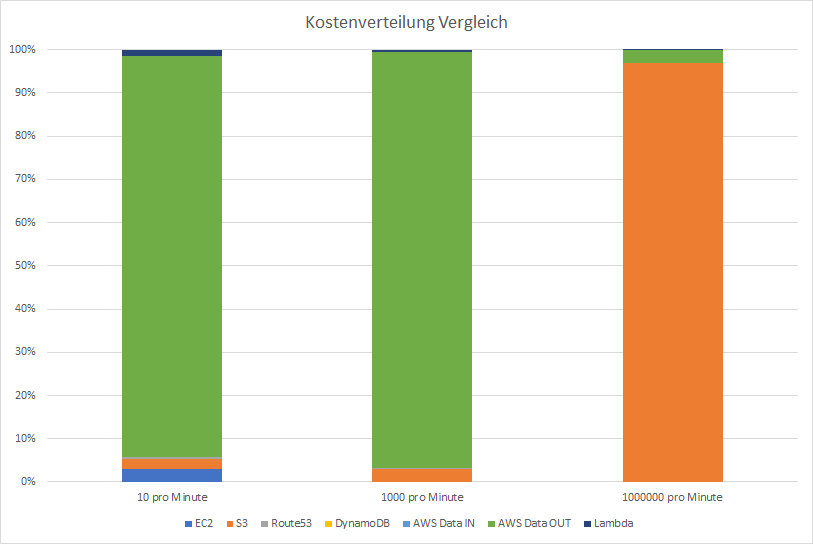
\includegraphics[scale=0.81]{costs-overview.png}
\caption{Kosten für 1000 Requests pro Minute}
\end{figure}

%@TODO: Grafiken raussuchen zu Kosten
%\begin{figure}[h]
%\centering
%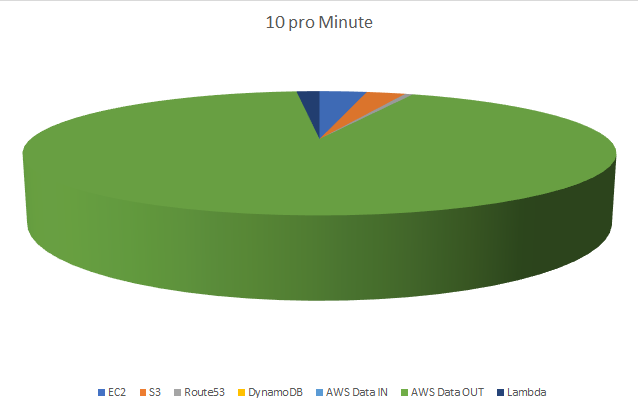
\includegraphics[scale=1]{costs-10.png}
%\caption{Kosten für 10 Requests pro Minute}
%\end{figure}
%\begin{figure}[h]
%\centering
%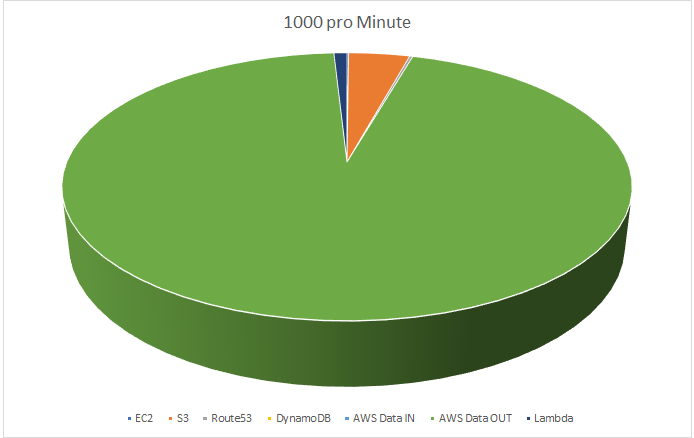
\includegraphics[scale=1]{costs-1000.png}
%\caption{Kosten für 1000 Requests pro Minute}
%\end{figure}
%\begin{figure}[h]
%\centering
%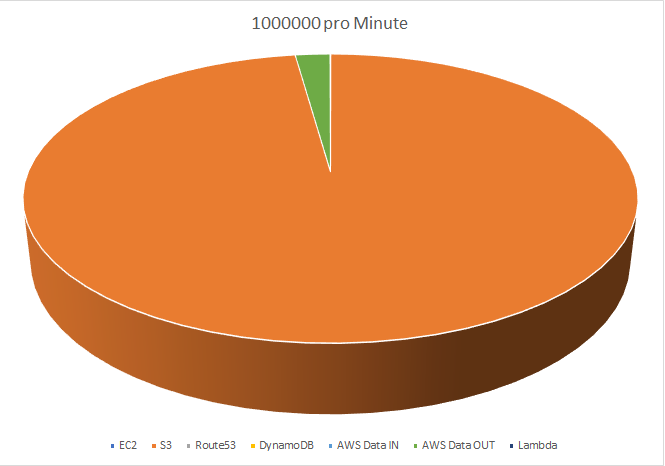
\includegraphics[scale=1]{costs-1000000.png}
%\caption{Kosten für 1000000 Requests pro Minute}
%\end{figure}

\subsection{Bewertung}
Wie man erkennen kann, ist aus Kostengründen bei einer sehr großen Filesharing Plattform (> 10.000 Aufrufe pro Minute) von unserer Umsetzung abzuraten. Die Kosten für den S3 Service wären untragbar. Denkbar wäre hier, wie später im Ausblick erwähnt, eine Umsetzung in \emph{Amazon Glacier.}\\
Interessanterweise ist die DynamoDB sehr \emph{günstig}, da die meisten Anfragen in einen freien Kontingent laufen und unsere Anfragen an die Datenbank sehr klein sind (<1KB). \\
Das verlagern des \textit{Speicherplatzproblems} von der EC2 Instanz nach S3 macht sich hier deutlich. Anstatt, dass die Kosten bei den EC2 Instanzen stark steigen, scheinen sie exponentiell im S3 Service zu steigen. Dies zeigt, dass wir für unsere Anwendung versucht haben möglichst viel aus der EC2 Instanz auszulagern. \\
Dank unseren schlanken Lambda Service, läuft dieser nur knapp 2 Sekunden und verbraucht <256Mbyte Arbeitsspeicher. Dadurch bleiben die Kosten überschaubar. Es ist dennoch interessant, dass sie bereits ab 1000 Aufrufen pro Minute die Kosten für die EC2 Instanzen übersteigen. 


%10 = https://calculator.s3.amazonaws.com/index.html?lng=de_DE#key=calc-2F0F41AC-C39D-4904-B349-2E27EC03B134&r=FRA
%1000 = https://calculator.s3.amazonaws.com/index.html?lng=de_DE#key=calc-D5DAB655-81D7-4FD6-B3D3-449FBD41FFC5&r=FRA
%1000000 = https://calculator.s3.amazonaws.com/index.html?lng=de_DE#key=calc-77814ED1-00F9-4058-8401-E0D1D464D215&r=FRA


%QUELLE LAMBDARECHNER
%https://dashbird.io/lambda-cost-calculator/
%QUELLE AWSRECHNER
%https://calculator.s3.amazonaws.com

\chapter{Ausblick}
Im Zuge einer Weiterentwicklung haben wir folgende Punkte gefunden, wodurch man den Funktionsumfang oder die Kosten bei AWS reduzieren könnte. Durch unser ständiges Augenmerk bei der Entwicklung auf Erweiterbarkeit, sollte es recht einfach sein unseren Code zu erweitern. \\
Folgende Punkte bieten Ausbaupotential:
\begin{itemize}
\item Wir haben eine eigene EC2 Instanz auf einen ElasticBeanstalk anstatt Lambda Funktionen gewählt, auch weil wir vor hatten Sockets zu implementieren. Diese Sockets würden den Nutzer die Möglichkeit geben Änderungen auf einen geteilten Desktop live zu sehen. 
\item Dank unserer vorausschauenden Programmierstruktur, haben wir die Funktionen die aufgerufen werden können wie, Auflisten der Elemente im Desktop, Auflisten der verschiedenen Desktops usw. möglichst weit gekapselt. Dadurch wäre der komplette Umbau auf Lambda theoretisch möglich. Dennoch würden wir keinen kompletten Umstieg auf Lambda empfehlen, da es auch Gründe gibt die bei manchen Funktionen dagegen spricht. Wie zum Beispiel das feste Lambda-Limit der Zeitüberschreitung von 15 Minuten. Ein Up- oder Download bei großen Dateien kann aber auch über 15 Minuten dauern und würde dann zum Abbruch führen.
\item Ein relativ einfaches Feature, dass man hinzufügen könnte wäre das hinzufügen eines SSL Zertifikates zu der EC2 Instanz beziehungsweise zum Route53 Service, um das Surfen über verschlüsselte Aufrufe über https zu ermöglichen. 
\item Gerade bei der Kostenoptimierung wäre ein direkter Zugriff auf die S3 Daten von Vorteil. Wie man in unserer Übersicht der Betriebskosten sieht ist dieses \emph{durchschleusen} ein großer Kostenfaktor. AWS bietet an mit speziellen \glqq Whitelist\grqq  Cookies Nutzer direkt auf die S3 Daten zugreifen zu lassen, auch bei Streams.
\item Ein weitere Idee die Kosten zu verringern, wäre die Nutzerdaten auf keinen S3-Bucket zu lagern sondern auf den AWS-Glacier. Dieser verspricht geringere Kosten bei vielen Datenmengen.
\item Auch das verlagern des Thumbnailservices in die ständig laufenden EC2 Instanzen würden die Kosten für den Lambda Service einsparen.
\item Das Setup Script nimmt zur Zeit Parameter entgegen, diese können auf einem unix system mit zum beispiel dem komandozeilenbefehl "top" von anderen Nutzern eingesehen werden, da die Parameter die AWS credials beinhalten, sollte das script so angepasst werden das diese aus der credials datei von aws ausgelessen werden (wie auch die aws-cli) bwziehungsweise die credials innerhalb der anwendung vom benutzer abgefragt werden.
\end{itemize}


\clearpage
\bibliographystyle{alpha}
\bibliography{documentation}
%\bibliographystyle{apalike}

\end{document}